\suppnote{Anisotropy and matched-capacity media}{note:spatial}

\paragraph{Local tensors and axial orientation.} For each regular interior cell, $\Lc$ maps signed face flux to two physical components. Define
\begin{equation}
\begin{aligned}
 \SigC(c)&=\Lc\CR\CR^\top\Lc^\top,\\
 \SigU(c)&=\Lc\UR\UR^\top\Lc^\top,\\
 A(c)&=\begin{cases}
 (\lambda_1(c)-\lambda_2(c))/(\lambda_1(c)+\lambda_2(c)),&\lambda_1(c)+\lambda_2(c)>0,\\
 0,&\lambda_1(c)+\lambda_2(c)=0 .
 \end{cases}
\end{aligned}
\label{eq:supp-local-tensors}
\end{equation}
Here $\lambda_1\ge\lambda_2$ are eigenvalues of the relevant tensor. The principal eigenvector defines an axis $\theta$ modulo $\pi$, not a directed arrow. San Francisco uses per-cell mean anisotropy and a nematic mean of $e^{2i\theta}$ over five folds. Directional coherence is
\begin{equation}
 S_{\mathrm{nem}}=\frac{\left|\sum_cw_c\AC(c)e^{2i\theta_C(c)}\right|}
 {\sum_cw_c\AC(c)},
 \label{eq:supp-nematic}
\end{equation}
with $w_c=1$ or $w_c=\tr\SigC(c)$.

Structural-axis agreement is the joint-anisotropy estimand
\begin{equation}
 G_\theta=\frac{\sum_c\AC(c)\AU(c)\cos[2(\theta_C(c)-\theta_U(c))]}{\sum_c\AC(c)\AU(c)},
 \qquad \AC(c)\AU(c)>0 ,
 \label{eq:supp-axis-agreement}
\end{equation}
on regular interior cells for which both anisotropies are nonzero. Because $\SigC$ uses a unit input metric, we also evaluate the source-covariance-weighted response tensor
\begin{equation}
 \Sigma_{\mathrm{response}}(c)=\Lc\CR\Sigma_{xx}\CR^\top\Lc^\top,
 \label{eq:supp-source-metric}
\end{equation}
with $\Sigma_{xx}$ the TRAIN covariance of source departures. Median anisotropies under this metric are 0.766, 0.926 and 0.765 in Porto, San Francisco and Chengdu, compared with 0.635, 0.651 and 0.705 under the unit metric. Strong local anisotropy persists under source-covariance weighting, indicating that directional selectivity is also pronounced under the realized excitation statistics. This comparison does not establish independence from every possible input metric.

Axis agreement is a separate question because $\CR$ and $\UR$ share the road subspace by construction. We write $K_R=Q\Lambda V^\top$ and replace $Q$ by a Haar-random orthonormal frame $Q_0$ in the road output space, $K_0=Q_0\Lambda V^\top$, preserving the spectrum and input directions. Recomputing $G_\theta$ for 999 draws gives null minima of 0.967, 0.902 and 0.803 and medians of 0.973, 0.911 and 0.808 in Porto, San Francisco and Chengdu. The archived estimates (five-fold consensus for San Francisco), 0.79, 0.79 and 0.76, lie below every null draw, so no observed value exceeds the null (one-sided empirical $p=1.0$ in all three cities). The archived tensors in \path{results/frozen/anisotropy/fo4_fig5_data.npz} and \path{results/frozen/anisotropy/chengdu_anisotropy.npz} are the single primary source for these estimates and for Fig.~\MainRef{fig:road-tests}a--c. Because the rotation requires $K_R$, which is not stored with those tensors, the null is generated by a control refit at the archived $\kappa$ and a single-fold reconstruction (San Francisco fold 0). This control reproduces the archived scale but is not used as an estimate; the reported conclusion uses only the archived estimates against the null quantiles, and the provenance audit records both the archived sources and the control's role. Because the control's own \(G_\theta\) is at least as large as the archived estimate in every city, the comparison is conservative for the reported conclusion. Axis agreement is not distinguishable from the spectrum-matched null and provides no independent evidence of a road-aligned response. We retain only the anisotropy magnitude as an operator property.

On the regular interior grids $\Lc\Lc^\top=2I$, so metric whitening is a no-op and grid anisotropy vanishes there; anisotropic boundary-cell metrics are excluded. An orthogonal road-coordinate rotation leaves the physical tensor unchanged when basis and coefficients are transformed together. Under a rigid physical rotation $Q$,
\begin{equation}
 \SigC(c)\mapsto Q\SigC(c)Q^\top,\qquad v_C(c)\mapsto Qv_C(c),
\end{equation}
while eigenvalues and scalar anisotropy are invariant. The axial vector is covariant, not numerically unchanged in fixed physical coordinates.

\begin{figure}[!htbp]
\centering
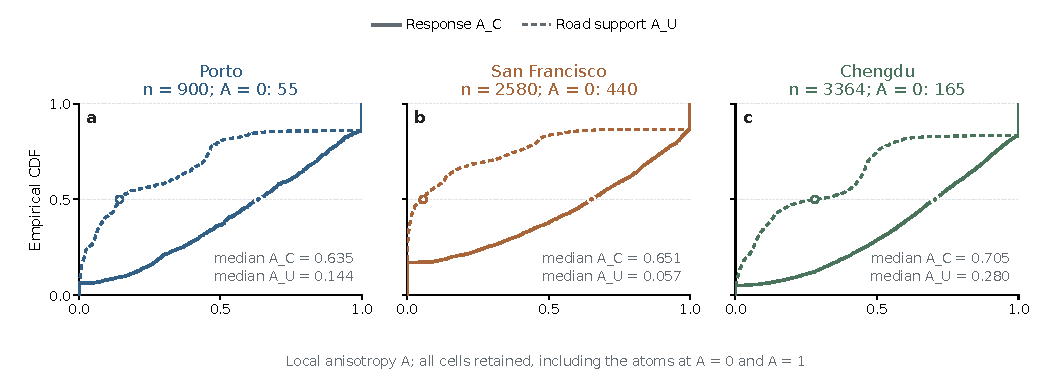
\includegraphics[width=0.72\textwidth]{figS04_anisotropy_distributions.pdf}
\caption{\textbf{Three-city local anisotropy distributions.} Empirical cumulative distribution of $A=(\lambda_1-\lambda_2)/(\lambda_1+\lambda_2)$, with $A=0$ assigned to a zero tensor, over regular interior cells for road support $\AU$ (dashed) and fitted response $\AC$ (solid); circles mark medians. Both curves use the same cells and per-cell definition. Endpoint steps are real atoms: cells without directional energy enter at $A=0$ (5--17\%, identical cell sets for $\AU$ and $\AC$), and one-dimensional tensors enter at $A=1$ (6--16\%). They are not normalization artefacts.}
\label{fig:supp-4}
\end{figure}

\paragraph{Matched-capacity media.} The compared media are a road medium from an external GIS raster, a mobility-inferred medium estimated from TRAIN mobility observations, and a permuted mobility medium. At capacity $R$, each per-face source pattern is averaged over $R$ spatial blocks and passed through the verified mean-1/floor normalization
\begin{equation}
 w^{(R)}_{S,f}=\max\!\left(\frac{\overline W^{(R)}_{S,f}}{\langle\overline W^{(R)}_S\rangle_{\mathrm{interior\ faces}}},\,0.02\right),
 \label{eq:supp-medium-normalization}
\end{equation}
before the archived minimum-energy field lift. Thus $R$ is the nominal number of block values before normalization, not the effective degrees of freedom: mean-1 normalization removes at least one independent degree, and the floor can reduce it further. With $R=1$ every medium is constant, and $R=n_{\mathrm{int}}$ assigns one pre-normalization value per interior face. Permutation preserves the mobility medium's values, partition and nominal block count while permuting its spatial arrangement. Road and mobility media do not have identical information inputs; equal $R$ matches capacity, not information.

The score is computed per held-out date against that date's own target mean and then averaged with equal date weight:
\begin{equation}
 R^2_{\mathrm{cond},d}=1-\frac{\sum_{t\in d}\norm{T_t-\widehat T_t}^2}{\sum_{t\in d}\norm{T_t-\langle T\rangle_d}^2}.
 \label{eq:supp-conditional-score}
\end{equation}
It is an archived date-centred statistic on the raw routing target, not on D's TRAIN-phase departure target, and is distinct from P and D in Eq.~\ref{eq:supp-pd-scores}. Figure~\ref{fig:supp-5} reports gains over the constant $R=1$ medium.

The nested grids are Porto $R=(1,4,16,64,256,1984)$ with block sides $(0,16,8,4,2,1)$; San Francisco $R=(1,3,12,44,176,704,5512)$ with block sides $(0,32,16,8,4,2,1)$; and Chengdu $R=(1,4,16,64,225,900,7080)$ with block sides $(0,32,16,8,4,2,1)$. Side zero denotes the single constant block. The final identity partition gives $R=n_{\mathrm{int}}=(1984,5512,7080)$. San Francisco uses its occupancy-defined channel and per-fold basis; Chengdu has only the archived all-motion channel and uses the frozen per-fold-basis rule on its chronological 10/4/4 split.

\begin{figure}[!htbp]
\centering
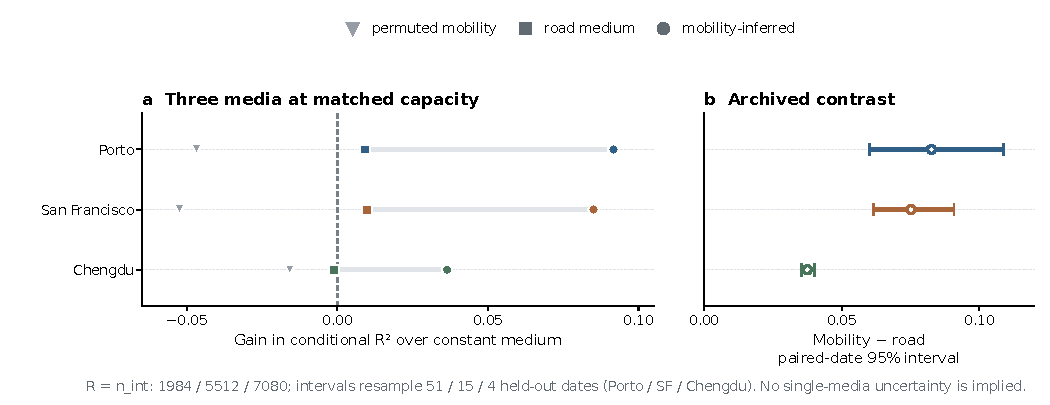
\includegraphics[width=0.68\textwidth]{figS05_matched_capacity.pdf}
\caption{\textbf{Three-city media at matched capacity.} Gain in held-out conditional $R^2$ over the constant $R=1$ medium for the permuted mobility medium, road medium and mobility-inferred medium at $R=n_{\mathrm{int}}$ (1984, 5512 and 7080 nominal pre-normalization block values). The score is the equal-date mean of within-date conditional $R^2$, distinct from P and D. Constant-medium values are 0.613, 0.743 and $-0.030$. Permutation preserves values, partition and nominal block count. Chengdu resamples four alternate-hour dates on a single all-motion channel; its points are small-sample summaries.}
\label{fig:supp-5}
\end{figure}

The matched-capacity modules \texttt{domain\_lib.py} and \texttt{domain\_rankmatched.py} are included in the public export, together with the sweep wrapper. The sweep still requires external aligned fields, date-freeze files and GIS rasters, which are listed with hashes in the data manifest; the archived passing-cell record validates the frozen run and is not a claim that the sweep runs without those inputs.
